\section{Some Examples}

\subsection{Tables}

Notice the missing | and \verb|\hline| in the \verb|chapter2.tex| file and their effects.

% If you don't need a caption/label you can remove the table environment.
\begin{table}[H]
    %\centering
    % Table captions should go above their tables, according to XAMK guidelines
    \caption{An example table} % \citecaption can also be used in tables
    \label{tab:tabletest}
    % extra | before first l and missing | after the last l
    \begin{tabular}[b]{ || l | l  }
    	\hline % "\\" adds a linebreak, "\hline" adds a horizontal line
    	Measurement 1 & $(20.49 \pm 0.01)\si{mm}$ \\\hline
    	Measurement 2 & $(20.47 \pm 0.01)\si{mm}$ \\%\hline
    	Measurement 3 & $(18.63 \pm 0.01)\si{mm}$ \\\hline
    \end{tabular}
\end{table}

\subsection{Mathematics}

% For physics units, \si{} can be used to distinguish units from variables (variables are italic).
% The "&"s control alignment. Try moving them around to adjust alignment.
\begin{align*}
    % _{} is used for subscript, ^{} is used for superscript
	V_{cuboid} &= w h l = 20.49\si{mm} \times 20.47\si{mm} \times 18.63\si{mm} \approx 7814\si{mm^{3}} \\ 
	% Notice how this \num{} converts its input into scientific notation
	G &= \num{6.673e-11}\si{N.m^{2}.kg^{-2}} \\ 
	% \num{} can also add those small spaces in large/small numbers
	\num{1000000} &= \num{1000000000000} \times \num{0.000001} \\
	% Calculus
	x &= \frac{-b \pm \sqrt{b^2 - 4ac}}{2a} \\
	\int_{x^2 + y^2 \leq R^2} & f(x,y)\,dx\,dy
	    = \int_{\theta=0}^{2\pi} \int_{r=0}^R f(r\cos\theta,r\sin\theta) r\,dr\,d\theta. \\
    % Matrices ("&" doesn't control alignment from within the matrix environment)
    \begin{bmatrix} 1 & 2 & 3 \\ 4 & 5 & 6 \end{bmatrix}&
        \begin{bmatrix} 7 & 8 \\ 9 & 10 \\ 11 & 12 \end{bmatrix} =
        \begin{bmatrix} 58 & 64 \\ 139 & 154 \end{bmatrix}
	% If \\ was included after the last row it'd create an extra empty line of space below
\end{align*}
% Empty lines should be avoided around an align* environment, to preserve page space.
% Alternatively, a comment (even a "%" by itself) can be used.

\subsection{Graphics}

It's a cube with a hole through the top. Try changing the value of \texttt{cubex}.

% If you don't need the caption/label you can remove the figure environment.
\begin{figure}[H]
    %\centering
    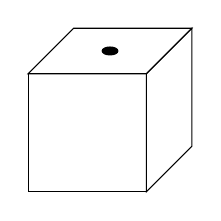
\begin{tikzpicture}
        \pgfmathsetmacro\cubex{1.5}
        \pgfmathsetmacro\cubey{1.5}
        \pgfmathsetmacro\cubez{1.5}
        \draw (0,0,0) -- ++(-\cubex,0,0) -- ++(0,-\cubey,0) -- ++(\cubex,0,0) -- cycle;
        \draw (0,0,0) -- ++(0,0,-\cubez) -- ++(0,-\cubey,0) -- ++(0,0,\cubez) -- cycle;
        \draw (0,0,0) -- ++(-\cubex,0,0) -- ++(0,0,-\cubez) -- ++(\cubex,0,0) -- cycle;
        \pgfmathsetmacro\circlex{\cubex/2}
        \pgfmathsetmacro\circlez{\cubez/2}
        \draw[fill=black] (-\circlex,0,-\circlez) ellipse (0.1 and 0.05);
    \end{tikzpicture}
    \citecaption{cube}{A cube drawn with TikZ}
    \label{fig:cube}
\end{figure}

\subsection{Graphs}

% If you don't need the caption/label you can remove the figure environment.
\begin{figure}[H]
    %\centering
    \begin{tikzpicture}
    % Google "pgfplots gallery" to see examples of graphs and how to make them.
    % If you need negative numbers, add the "axis lines=middle" option to axis.
    \begin{axis}[
    xmin=0, xmax=1.2, ymin=0, ymax=2, % sets x-axis and y-axis limits
    xlabel={foo $a_1$ (\si{m.s^{-2}})}, % set x axis label
    ylabel={bar \\ $a_2$ (\si{m.s^{-2}})}] % set y axis label
    	\addplot+[only marks,error bars/.cd,
    	y dir=both,y explicit,
    	x dir=both,x explicit]
    	coordinates { % points
    		(0.1702, 0.376) +- (0.05, 0.25)
    		(0.2867, 0.552) +- (0.05, 0.25)
    		(0.3886, 0.724) +- (0.05, 0.25)
    		(0.4410, 0.891) +- (0.05, 0.25)
    		(0.5589, 1.05)  +- (0.05, 0.25)
    		(0.6659, 1.20)  +- (0.05, 0.25)
    		(0.7574, 1.35)  +- (0.05, 0.25)
    		(0.8580, 1.49)  +- (0.05, 0.25)
    		(0.9415, 1.63)  +- (0.05, 0.25)
    		(1.070,  1.77)  +- (0.05, 0.25)
    	};
    	% By default line domains are set to -5:5. You'll want to manually set them.
    	\addplot[domain=0:2, color=black, mark=none, dotted] {2.2*x}; % dotted line
    	\addplot[domain=0:2, color=black, mark=none, solid] {(1/0.541)*x}; % solid line
    	\addplot[domain=0:2, color=black, mark=none, dashed] {1.5*x}; % dashed line
    \end{axis}
    \end{tikzpicture}
    \caption{A graph using TikZ's axis environment}
    \label{fig:fancygraph}
\end{figure}

\subsection{Monospace text}

Some inlined paths: \lstinline{C:\Windows}, \lstinline{~/.bashrc} % \verb|| works as well

% Settings within square brackets "[]" are optional.
% The $, #, and space characters must be escaped to work properly.
\begin{cmd}[title={Some command-line commands},label=code:linux-cmd,every listing line={\$\#>\ }]
wget http://tex.stackexchange.com
echo "is this thing working?" > test.txt
\end{cmd}

% The starting line number is set with minted's "firstnumber".
% {python} sets the language, see https://pygments.org/docs/lexers/ for the language list.
\begin{code}[firstnumber=11]{python}[title={Some Python code with syntax highlighting},label=code:python-eg]
def zip_gen(tuple_list):
    for index in range(min(len(tuple_list[0]), len(tuple_list[1]))):
        yield {tuple_list[0][index]: tuple_list[1][index]}
\end{code}

\begin{comment} % This section is hidden due to the comment environment
Some C-sharp code with syntax highlighting:
% {csharp} sets syntax highlighting to C#.
\begin{code}{csharp}
private void StoreItemClicked(object sender, SelectionChangedEventArgs e) {
    if(Store.SelectedIndex != -1) {
        booksInCart.Add(booksInStore[Store.SelectedIndex]);
        booksInStore.RemoveAt(Store.SelectedIndex);
    }
    Refresh_ListBoxes();
}
\end{code}
\end{comment}

\subsection{Images}

A figure containing an image and a caption:
% Figures (and tables) will reorder your layout if they're forced onto the next page.
% Using the [H] option for all figures and tables should prevent this problem from occurring.
% You could also manually reduce a figure's width or scale to fit within its page.
% If you don't need a caption/label for a figure you can use just the \includegraphics command.
\begin{figure}[H]
	%\centering % Uncomment to center the image and its caption
	% The image is scaled to 80% of the page's line width
	
\includegraphics[width=0.8\linewidth]{LaTeX-logo.png}
	\citecaption{latex-logo}{The \LaTeX\ logo}
	\label{fig:latex-logo}
\end{figure}
